\chapter{Discussion}

\label{chapter:discussion}

\rem{Il faut discuter du parti pris dans mon scénario : c'est de croire que mu D alpha c'est toujours bon pour le alpha ROM et que ce qui change c'est juste ...}

\subparagraph{}Dans ce chapitre, nous proposons de rassembler les résultats obtenus dans les chapitres précédents afin de mener une étude comparée de la transition de réversibilité et de la transition vers l'écoulement. Nous nous appuierons tout d'abord sur les modèles numériques étudiés pour formuler plus précisément l'analogie entre des deux systèmes, du point de vue microscopique comme du point de vue de modélisation en champ moyen. Nous montrerons alors l'importance donnée aux mécanismes de bruit interne présents dans ces deux phénomènes.

\subparagraph{}Nous comparerons ensuite les évolution mesurées dans les modèles numériques de la criticalité de ces transitions avec la portée de l'interaction. Si celles-ci suivent des évolutions globalement similaires, nous montrerons comment expliquer les points de divergence qu'elles présentent via les ingrédients de la dynamique présents dans les modèles microscopiques.

\subparagraph{}Enfin, nous ouvrirons notre étude commune de ces deux phénomènes sur une piste de compréhension globale des transitions convexes présentant un mécanisme de diffusion. Via l'intégration numérique d'équations de champ associées, nous mettrons en avant les difficultés que pose une telle formulation continue de ces phénomènes.

\section{Comparaison des transitions étudiées}

\subsection{Similarités globales}

\subsubsection{Analogie entre les deux systèmes}

\subparagraph{}Après avoir présenté une étude exhaustive des deux transitions via les modèles numériques évoqués aux chapitres précédents, nous proposons de revenir sur les conclusions du chapitre d'introduction, pour reformuler plus précisément l'analogie entre les deux systèmes. Dans le \autoref{tab:analogie}, nous développons les parallèles réalisables entre ces deux transitions représentées par les modèles du $\alpha$-ROM et du $\alpha$-Picard.

\paragraph{Activité et quantité conservée}

\subparagraph{}\`A l'instar des modèles appartenant à la classe CDP, les modèles $\alpha$-ROM et $\alpha$-Picard font tout deux intervenir la dynamique d'une activité et d'une quantité conservée. Concernant la quantité conservée, elle correspond à la contrainte locale $\sigma(\mathbf{r},t)$ dans les modèles d'écoulement, qui est l'équivalent de la densité de particules $\rho(\mathbf{r}, t)$ dans les modèles de réversibilité. Cette première analogie rappelle directement le parallèle entre transition de dépiégeage et modèles de particules dans la classe CDP. Du côté de l'activité, une analogie directed est établie entre l'activité gros grains $A(\mathbf{r}, t)$ dans le $\alpha$-ROM et la variable locale $\dot{\epsilon}_\text{pl}(\mathbf{r}, t)$ dans le modèle élastoplastique.

\subparagraph{}Dans les deux cas, et comme dans tous les modèles représentés par l'universalité CDP, la valeur locale du champ conservé correspond en quelques sortes à une susceptibilité à l'activation. Une densité élevée dans le $\alpha$-ROM correspond à des particules proches, i.e. susceptibles de se recouvrir suite à un petit déplacement et donc de créer de l'activité. Dans le modèle $\alpha$-Picard, une contrainte locale élevée représente une faible distance au seuil microscopique $\sigma_Y$ et donc une éventualité forte de devenir plastique en la présence de fluctuations externes.

\subparagraph{}D'un point de vue macroscopique, les paramètres de contrôle homologues l'un de l'autre sont la contrainte globale $\Sigma$ et la densité globale $\phi$, tandis que l'équivalence des paramètres d'ordre se retrouve via la proportion moyenne de particules actives $\langle A \rangle $ et le taux de cisaillement moyen $\langle \dot{\gamma}\rangle$.

\paragraph{Avalanches et hyperuniformité}

\subparagraph{}Comme les autres modèles appartenant à la classe CDP, le $\alpha$-ROM et le modèle $\alpha$-Picard présentent des dynamiques d'avalanche proche du point critique, que nous avons mis en évidence dans des conditions de contrainte/densité imposée. En accord avec les équivalences précédentes, là où la taille d'une avalanche dans le modèle $\alpha$-Picard est représentée par le déplacement global du matériau, celle dans le $\alpha$-ROM correspond à la quantité d'évènements actifs qui la constituent. De même, on retrouve dans ces deux systèmes, dans une certains limite, la propriété d'hyperuniformité. Si celle-ci se traduit dans le modèle de particules via les fluctuations anormales de densité, dans le modèle d'écoulement elle correspond aux fluctuations anormales de contrainte.

\paragraph{Effets multiples des évènements d'activité}

\subparagraph{}Les deux familles de modèles présentent aussi une analogie claire via l'effet d'un évènement actif. Celui-ci peut en fait être découpé en trois contributions : un effet de relaxation, un effet de transport et un effet non-local spécifique. Nous verrons que ce découpage est utile pour comprendre les différents mécanismes à l’œuvre dans chacune de ces transitions. Prenons tout d'abord le cas du $\alpha$-ROM. Le processus de relaxation se traduit dans ce cas par le saut de la particule active qui défait le recouvrement : c'est un processus d'auto-inhibition local de l'activité. D'autre part, le processus de transport, qui représente le mécanisme classique de propagation de l'activité dans les modèles appartenant à la classe CDP, correspond au déplacement de la particule active qui est susceptible d'en recouvrir une autre. Enfin, le processus non-local spécifique, qui le différencie des autres modèles, est l'interaction entre particules actives et passives à longue portée, représentée par des petits déplacements des particules passives sans transport des particules actives. 

\subparagraph{}Dans le cas du modèle d'écoulement, ce découpage est un peu moins évident mais peut être compris par une ré-écriture formelle du propagateur selon :

\begin{equation}
	G(\mathbf{r}-\mathbf{r}^\prime) = G(0) + G_1(\mathbf{r}-\mathbf{r}^\prime) + G_2(\mathbf{r}-\mathbf{r}^\prime), \quad G_1(\mathbf{r}) > 0, \quad \int \mathrm{d}\mathbf{r}~ G_1(\mathbf{r}) = -G(0)
\end{equation}

\noindent Dans ce cadre, le processus de relaxation correspond à la partie $G(0)<0$ du propagateur qui traduit la relaxation d'un site plastique, l'amenant vers $\sigma < \sigma_Y$. Le processus de transport, quant à lui, correspond à la redistribution de cette contrainte relaxée via une partie positive du propagateur $G_1$. Dans le cas de la transition de dépiégeage, le propagateur élastique n'est formé que des deux premiers termes. La particularité du propagateur non-monotone d'Eshelby dans le cas de la transition vers l'écoulement fait intervenir un troisième terme $G_2$, à longue portée et de signe alterné. C'est cette partie qui représente l'effet non-local spécifique de la transition, absent des modèles représentant les classes CDP et LR-CDP.

\subparagraph{}L'ingrédient constitutif qui rapproche les deux transitions de réversibilité et d'écoulement et les sépare des classes CDP et LR-CDP est précisément cette partie non-locale spécifique de l'effet de l'activité. Dans la suite, nous rappelons brièvement en quoi celle-ci représente une nouveau mécanisme de création de l'activité.

\begingroup

\setlength{\tabcolsep}{10pt}
\renewcommand{\arraystretch}{1.5}

\begin{table}[h]
\centering
\begin{tabular}{P{0.25\linewidth}P{0.35\linewidth}P{0.35\linewidth}}
\hline \hline  & Transition de réversibilité & Transition vers l'écoulement \\
\hline
Param. de contrôle  & densité $\phi$ & contrainte $\Sigma$ \\
Param. d'ordre & fraction de particules actives $A$ & taux de cisaillement $\dot{\gamma}$ \\
Mise en activité & contact : $|\mathbf{r}-\mathbf{r}^\prime| < D_P$ & dépassement du seuil : $\sigma > \sigma_Y$\\
Effet local de l'act. & saut & relaxation de $\sigma$ \\
Effet non-local de l'act. & déplacement des part. passives & redistribution non-monotone de la contrainte \\
Distribution de distance micro.  & fonction de corrélation de paire : $g_p(|\mathbf{r}-\mathbf{r}^\prime|-D_p)$ & distribution de distance au seuil : $P(\sigma_Y - \sigma)$\\
\hline 
Présence de transport à longue portée & Non & Oui \\
Géométrie du propagateur & isotrope & présence de modes 0 \\
\hline \hline
\end{tabular}
\caption{Tableau d'analogie entre la transition de réversibilité et la transition vers l'écoulement étudiées via les modèles $\alpha$-ROM et $\alpha$-Picard.}
\label{tab:analogie}
\end{table}

\endgroup

\subsubsection{Bruit interne, bruit mécanique}

\paragraph{Diffusion et bord absorbant}

\subparagraph{}Dans le modèle $\alpha$-ROM, comme nous l'avons discuté au \autoref{chapter:Susp}, l'effet non-local spécifique des interactions à longue portée provoque une diffusion des particules passives via l'effet successif de nombreux évènements actifs. Cette diffusion représente alors un mécanisme de propagation de l'activité très différent de celui des modèles associés à la classe CDP. Sous l’influence du bruit interne, les particules passives se déplacent aléatoirement et finissent par se rencontrer. Ainsi, à partir de deux particules passives, deux particules actives sont créées, tandis que les particules actives à l'origine de ce bruit interne poursuivent leur dynamique locale. Formellement, ce mécanisme de création de l'activité peut être associé à une marche aléatoire en présence d'un bord absorbant. Dans le modèle de suspensions, pour une particule passive, toute autre particule représente ce bord absorbant. L'absorption de la particule correspond alors à un évènement d'activité.

\subparagraph{}Le même constant peut être fait du point de vue des modèles élastoplastiques en considérant l'effet de la partie $G_2$ du propagateur. Si l'on se concentre sur un site élastique lors d'un pas de temps unique, en fonction de sa position à la plasticité, sa contrainte locale se voit augmenter ou diminuer de manière plus ou moins importante. Au cours de l'écoulement, via les fluctuations de plasticité dans le système, la contrainte locale de ce site va donc fluctuer de manière pseudo-aléatoire. Dans ce cadre, nous pouvons donc voir l'effet non-local spécifique de ces modèles comme induisant une diffusion des contraintes locales. Là encore, cette diffusion définit un nouveau mécanisme de création d'activité qui peut être compris comme une marche aléatoire en présence d'un bord absorbant. La contrainte locale $\sigma$ diffuse sous l'action de la plasticité jusqu'à arriver au seuil $\sigma_Y$ qui représente le bord absorbant, créant ainsi un évènement actif. 

\subparagraph{}Ces mécanismes de diffusion vers un bord absorbant sont complexes à appréhender en dimension finie car ils ne peuvent pas être réellement réduit à un problème de marche aléatoire simple. Dans le cas du $\alpha$-ROM, cela vient du fait que les particules actives qui créent le bruit interne opèrent une dynamique corrélée non-triviale et que la notion de bord absorbant ne renvoie pas à une frontière fixe mais à un ensemble de particules diffusant elles aussi dans une espace de dimension finie. Dans le cas du modèle $\alpha$-Picard, l'effet du propagateur $G_2$ n'est que pseudo-aléatoire puisqu'il présente une forte anisotropie quadrupolaire en plus d'une spatialisation. Pour ces raisons, il est plus simple d'aborder ce mécanisme via un point de vue champ moyen qui permet de s'affranchir de toutes ces sources de complexité. 


\paragraph{Modélisation champ moyen}

\subparagraph{}Il est possible d’interpréter les deux transitions via des modèles de champ moyen comprenant ce mécanisme non-local spécifique de la manière la plus simple qu'il soit. Ceux-ci se démarquent des approches champ moyen issues des équations de champ comme dans le cas de CDP par deux aspects : l'objet central de la théorie est le champ conservé et non le champ d'activité, et le point de vue adopté est un point de vue statistique, via la dynamique effective d'un agent unique.

\subparagraph{}Dans le cadre de la transition vers l'écoulement, ce modèle champ moyen est le modèle de Hébraud-Lequeux \cite{hebraud_mode-coupling_1998}, décrit par l'équation :

\begin{equation}
\begin{aligned}
	\partial_t P(\sigma, t) &= -\dot{\gamma}(t)\partial_\sigma P(\sigma, t) + \alpha\Gamma(t)\partial_\sigma^2P(\sigma, t) - \frac{\Theta (|\sigma|>\sigma_Y)}{\tau}P(\sigma, t) + \Gamma(t)\delta(\sigma)\\
	\Gamma(t) &= \frac{1}{\tau}\int_{|\sigma|>\sigma_Y}\mathrm{d}\sigma ~ P(\sigma, t)
\end{aligned}
\end{equation}

\noindent avec $\dot{\gamma}(t) = \dot{\gamma}$ dans des conditions de taux de cisaillement imposé ou alors :

\begin{equation}
	\dot{\gamma} (t) = \frac{1}{\tau}\int_{|\sigma|>\sigma_Y}\mathrm{d}\sigma ~ \sigma P(\sigma, t)
\end{equation}

\noindent dans le cas où c'est la contrainte globale $\Sigma = \int \mathrm{d}\sigma ~ \sigma P(\sigma,t)$ qui est imposée.

\subparagraph{}Dans le cas de la transition de réversibilité, le modèle équivalent est décrit par les équations présentées au \autoref{chapter:Susp} :

\begin{equation}
    \partial_t P(\mathbf{r}, t) = \alpha\Gamma (t)\Delta P(\mathbf{r}, t) - \frac{1}{\tau}\Theta(|\mathbf{r}|>R)P(\mathbf{r}, t) + \delta(\mathbf{r})\Gamma (t), \quad \Gamma (t) = \frac{1}{\tau}\int_{|\mathbf{r}|>R}\mathrm{d}\mathbf{r}~P(\mathbf{r}, t)
    \label{eq:muHLDiff}
\end{equation} 

\subparagraph{}Là où le lien avec la modélisation élastoplastique est complètement transparent, celui avec le modèle de suspensions demande un certain degré d'abstraction et d'hypothèse via la mise en place d'une cage effective de dimension $R$, comme nous l'avons présenté au \autoref{chapter:Susp}. Ceci fait, les équations sont très similaires et permettent de comprendre les interactions à longue portée de la même façon via les termes en laplacien : chaque élément est soumis à un bruit dont l'intensité est proportionnelle à l'activité dans le système. Par ailleurs tout élément ayant dépassé le bord absorbant ($R$ ou $\sigma_Y$) est considéré comme actif.

\subparagraph{}La différence fondamentale entre ces deux modèles est la présence d'un terme de forçage en $\sim \dot{\gamma}$ dans le modèle de Hébraud-Lequeux, absent dans l'équivalent particulaire, et la dimension dans laquelle prend place la diffusion. Toutefois, en considérant les paramètres de contrôle respectifs ($\Sigma = \int \mathrm{d}\sigma ~ \sigma P(\sigma,t)$ dans le cas de la transition d'écoulement et $R$ dans le cas de la transition de réversibilité), ces deux modèles prédisent un même comportement critique représenté par un exposant $\beta = 2$ :

\begin{equation}
	\Gamma \sim (\Sigma - \Sigma_c)^2,\quad \Gamma \sim (R-R_c)^2
\end{equation}

\noindent Ces modèles renforcent alors l'analogie entre les deux transitions et placent ainsi le mécanisme de création de l'activité par diffusion comme l'explication de la convexité observée dans les modèles de dimension finie.

\paragraph{Extension à l'influence de la portée des interactions}

\subparagraph{}Comme on l'a vu dans le cas des suspensions au \autoref{chapter:Susp}, il est possible d’interpréter l'influence de la portée des interactions dans ce cadre champ moyen en considérant que celle-ci dicte les propriétés du bruit interne, plus précisément sa distribution. Cela se traduit dans les équations des modèles par un remplacement du laplacien classique $\Delta$ en un laplacien fractionnaire $\Delta^\mu$. Dans le modèle d'écoulement, cette généralisation a été étudiée précédemment par Lin et al. \cite{lin_mean-field_2016, lin_microscopic_2018}, montrant une évolution de la convexité avec $\mu$ décrite par :

\begin{equation}
	\beta = \left\{
	\begin{aligned}
	&2, \quad \mu > 2\\
	&\mu, \quad 1<\mu<2\\
	&1, \quad \mu < 1
	\end{aligned}
	\right.
\end{equation}

\noindent et la présence de corrections logarithmiques dans le cas limite $\mu = 1$\footnote{Dans ce cas là nous avons $\delta\Sigma \sim \dot{\gamma}\log(\dot{\gamma})$}. Dans l'approximation où le système est exempt de toutes corrélations liées à la dimension du système, l'équivalence discutée au \autoref{chapter:Susp} entre $\mu$ et $D/\alpha$ suggère que les interactions à longue portée dans un modèle 2D influent sur le comportement critique entre $\alpha = 2$ et $\alpha = 1$ avec $\beta$ passant de $\beta = 1$ à $\beta = 2$. Nous avons alors montré dans cet ouvrage que ces résultats se transposaient aussi au modèle champ moyen de particules, suggérant ainsi que l'influence de la portée des interactions est en principe le même dans les deux cas.

\subparagraph{}Ce cadre théorique qui permet d'expliquer l'évolution globale de la convexité sert alors d'appui pour interpréter les résultats obtenus dans les simulations de dimension finie et comparer plus quantitativement les deux transitions. C'est ce que nous ferons plus en détail à la \autoref{sec:Diff}.

\subsubsection{Répartition de la masse et distance à l'activation : des indices microscopiques}

\subparagraph{}En plus de de la convexité des transitions, une preuve de l'importance du mécanisme de diffusion vers la création d'activité dans les modèles $\alpha$-ROM et $\alpha$-Picard vient des distributions de distances à l'activation.

\subparagraph{}Dans le cadre champ moyen commun aux deux transitions, nous pouvons définir une distance à l'activation associée à la dynamique à agent unique étudiée. Dans le cas du modèle d'écoulement, cette distance à l'activation est la distance à la contrainte seuil $x = \sigma_Y - \sigma$. Dans le cas du modèle de particules, c'est la distance au bord de la cage effective $x = R-|\mathbf{r}|$. Proche de la transition, les modèles champs moyens prévoient une distribution algébrique de ces distances dictée par un exposant critique $\theta$ selon :

\begin{equation}
	P(x) \sim x^\theta, \quad \theta = \left\{
	\begin{aligned}
	&\frac{\mu}{2}, \quad 1 < \mu \leq 2\\
	&1, \quad \mu \geq 2
	\end{aligned}
	\right.
\end{equation}

\noindent et le cas $\mu \leq 1$ dépendant de la présence ou non d'un forçage dans le modèle \cite{lin_mean-field_2016} (et donc différent dans le cas du modèle d'écoulement et le modèle de particules). Ce résultat place alors la mesure $\theta > 0.5$ en témoin de l'importance du mécanisme de diffusion dans la transition.

\subparagraph{}Par construction, il est possible de définir un équivalent de ces propriétés dans les modèles microscopiques. Dans le modèle $\alpha$-Picard, l'équivalence est directe avec la distribution $P(x)$, $x$ étant la distance au seuil définie sur chacun des $N$ sites. Dans le $\alpha$-ROM, cette distribution correspond à un dérivé de la fonction de corrélation de paire entre particules passives $g_p(r - D_p)$.

\subparagraph{}Dans le cas du modèle de particules, nous avons montré que cette distribution était effectivement caractérisée par un exposant $\theta$ non-trivial évoluant avec la portée. Dans le cas du modèle élastoplastique, la quantité $P(x)$ a été étudiée à de nombreuses reprises, notamment car l'exposant $\theta$ est relié aux propriétés des avalanches quasistatiques \cite{lin_scaling_2014, ferrero_criticality_2019, liu_driving_2016, lin_mean-field_2016}. Dans ces études, on retrouve aussi dans le cas d'un propagateur de type Eshelby un exposant $\theta$ non-trivial entre $\theta = 0.5$ et $\theta = 1$. Notamment, dans le modèle de Picard que nous avons étudié, nous mesurons $\theta \approx 0.62$ (voir \autoref{sec:article2}). Cette propriété est un marqueur de la dynamique microscopique diffusive, abesente dans les modèles de type CDP et depinning pour lesquels on a $\theta = 0$\footnote{C'est ce que disent Lin et Wyart dans le PNAS mais est-ce qu'ils ne se contredisent pas après ?} et conforte donc l'interprétation de ces transitions via le cadre de champ moyen commun proposé.

\subsubsection{Évolutions mesurées des criticalités avec la portée des interactions}

\subparagraph{}Dans une certaine mesure, l'évolution mesurée des criticalités du $\alpha$-ROM et du modèle $\alpha$-Picard avec la portée d'interaction $\alpha$ sont très similaires. Dans les deux cas, on passe continûment d'un comportement de courte portée similaire (ou équivalent) à la classe CDP à un comportement de très longue portée, similaire à celui proposé par les modèles de champ moyen. Dans la limite de très longue portée, nous observons un comportement atypique dans les lois d'échelle régissant le régime stationnaire. L'évolution du paramètre d'ordre en fonction de la distance au point critique est convexe, caractérisée par un exposant $\beta$ proche de $2$, et les fluctuations de l'activité s'annulent à l'approche du point critique, carcatérisées par un exposant $\gamma^\prime$ négatif.

\subparagraph{}Cette atypicité se traduit aussi dans les propriétés dynamiques des transitions, plus particulièrement via la dynamique d'avalanche à contrainte/densité imposée dans la limite de longue portée. Dans ce cas, les évènements perdent leur compacité spatiale, avec une extension spatiale caractérisée par un exposant $\chi$ inférieur à la dimension de l'espace $\chi < D$. De plus, nous observons dans les deux modèles que dans cette limite, les exposants $\chi$ et la dimension fractale des avalanches $d_f$ sont liés trivialement par $d_f\approx \chi$. Le fait que la taille d'un évènement se comporte directement comme le nombre d'éléments impliqués suggère une sorte de trivialisation de la dynamique. L'évolution des propriétés critiques dynamiques repose alors essentiellement sur l'évolution de $\chi$ qui présente une perte de compacité supposée continue.

\subparagraph{}En fait, plus généralement, les évolutions de la plupart des exposants critiques prennent la même forme que celles dans le cadre de la théorie LR-CDP : en augmentant la portée des interactions l'évolution du paramètre d'ordre devient moins concave, les fluctuations divergent de moins en moins fortement, les avalanches sont de moins en moins compactes, etc ... Simplement, dans le cadre de ces deux transitions, la limite de longue portée est modifiée. Le mécanisme de diffusion vers l'activité permet d'aller au-delà du comportement champ moyen de la classe CDP.

\subparagraph{}Une observation remarquable est que dans les deux cas, ce passage aux propriétés anormales se fait de manière simultanée pour tous les exposants. En d'autres termes, la limite de la région atypique est un point correspondant sous presque tous les aspects au comportement champ moyen de la classe CDP. Dans le cas du modèle $\alpha$-Picard, ce point est retrouvé autour de $\alpha \approx 3$. Pour le modèle $\alpha$-ROM, c'est autour de $\alpha \approx 1.5$. Il est possible que des relations d'échelle sous-jacentes permettent de rationaliser en partie cette simultanéité. En revanche, il n'est toutefois pas clair qu'il existe une relation de cause à effet entre ces observations ou si elles représentent simplement une façon cohérente de caractériser cette dynamique. Quoiqu'il en soit, cette étude semble souligner le lien étroit entre convexité, évanescence des fluctuations et compacité de la dynamique. Dès lors, l'observation d'un élément de ce triptyque dans des systèmes différents pourrait suggérer la présence des deux autres propriétés, ou plus généralement la présence d'un mécanisme de diffusion vers l'activité.

\subsection{Différences en dimension finie}

\subparagraph{}Si les modèles $\alpha$-Picard et $\alpha$-ROM sont similaires sous bien des aspects, leur étude détaillée aux \autoref{chapter:Susp} et \autoref{chapter:yielding} révèle des différences entre ces deux phénomènes. Dans cette sous-section, nous reprenons les approches théoriques présentées dans cette thèse pour expliquer les différences apparentes entre la criticalité du modèle de suspensions et celle du modèle d'écoulement. Nous séparons ces différences, entre les deux modèles et entre les modèles et les approches théoriques, en deux catégories : celles de la zone concave $\beta < 1$ et celles de la zone convexe $\beta > 1$. Nous montrons alors que malgré ces divergences, l'interprétation de ces phénomènes dans un même cadre en dimension fini permet de mieux les appréhender.

\label{sec:Diff}

\subsubsection{Modèles d'appréhension théoriques}

\subparagraph{}Pour comprendre l'influence de la portée d'interaction sur le comportement critique dans les modèles $\alpha$-Picard et $\alpha$-ROM, nous disposons de deux approches théoriques. La première est celle présentée au \autoref{chapter:TransportLP}, baptisée LR-CDP, représentant l'influence d'un transport à longue portée. En 2D, celle-ci prévoit une évolution continue des exposants entre $\alpha = 4$ et $\alpha = 3$, avec l'exposant $\beta$ allant de $\beta \approx 0.64$ à $\beta = 1$. La seconde est celle des modèles $\mu$-Hébraud-Lequeux qui, comme nous l'avons rappelé juste avant, prédisent une évolution continue de la criticalité entre $\alpha=2$ et $\alpha = 1$ en 2D avec $\beta$ allant de $\beta = 1$ à $\beta = 2$. Nous représentons à la \autoref{fig:Recap}-(a) la combinaison de ces deux approches qui opèrent sur des domaines disjoints. Nous proposons alors de comparer les évolutions mesurées dans le $\alpha$-ROM et dans le $\alpha$-Picard sur cette base.

\subsubsection{Zone concave : des évolutions décalées}

\subparagraph{}En comparant la \autoref{fig:Recap}-(b) et la \autoref{fig:Recap}-(c), une première différence est frappante : la gamme de portées pour laquelle la transition est concave n'est pas la même dans les deux cas. Dans le cas du modèle $\alpha$-Picard, celle-ci est définie par $\alpha \gtrsim 3$, avec une évolution très proche de celle du cadre LR-CDP, alors que dans le $\alpha$-ROM elle correspond à $\alpha \gtrsim 1.5$, montrant une évolution plus abrupte.

\subparagraph{}La différence de principe fondamentale entre les deux modèles qui explique le décalage de ce début d'évolution est à chercher du côté des propriétés de transport. Dans le cadre LR-CDP, l'évolution continue de la criticalité résulte d'une redstribution de masse (ou de contrainte) qui se fait à une portée de plus en plus étendue. Dans le modèle $\alpha$-Picard, cette propriété se retrouve dans la partie $G_1$ du propagateur qui correspond au transport de la contrainte localement relaxée, évoluant comme $\sim 1/r^\alpha$. Ceci explique l'accord qualitatif avec la théorie LR-CDP. En revanche, dans le $\alpha$-ROM, la redistribution de masse suite à un évènement actif est toujours à courte portée : une particule active saute uniquement dans son voisinage. Ainsi, il n'est pas question de transport à longue portée dans le modèle de particules. C'est la raison pour laquelle la criticalité est invariante dans la zone $\alpha > 3$ associée à LR-CDP.

\subparagraph{}Le mode de transport étant absent dans le cadre du $\alpha$-ROM, le seul mécanisme susceptible de modifier le comportement critique est le bruit interne. C'est pourquoi le début d'influence de la portée d'interaction sur la criticalité est retrouvé à $\alpha \approx 2$, en accord avec le cadre théorique $\mu$-HL.

\subparagraph{}En d'autres termes, alors que la partie concave du modèle d'écoulement correspond à une extension de la dynamique à longue portée, celle du modèle de particules correspond à l'introduction du mécanisme de bruit interne en superposition de la dynamique locale pré-existante. Dans ce deuxième cas, le comportement critique résulte donc d'une interaction complexe entre les deux mécanismes. Ceci permet d'expliquer une première différence entre le modèle de particules et la théorie $\mu$-HL : le fait que la dynamique active ne soit pas trivialisée en $\alpha = 2$ fait que l'influence du bruit interne démarre à $\beta \approx 0.64$ et non $\beta = 1$ avant de l'amener autour de $\beta \approx 2$. Cette différence est illustrée par le texte \textit{corrélations (actives)} sur la \autoref{fig:Recap}-(b), puisque c'est la dynamique non-triviale sous-jacente des particules actives qui justifie cet écart avec la théorie. Ainsi, dans ce cas, c'est le bruit interne qui permet d'effacer la concavité de la transition.

\subparagraph{}Cette différence permet de mieux comprendre les mesures d'hyperuniformité réalisées au \autoref{chapter:Susp} et au \autoref{chapter:yielding}. Dans le cas de la transition vers l'écoulement, les évolutions de l'hyperuniformité avec la portée étaient clairement définie par un exposant critique $\alpha_\text{HU}$ évoluant de la manière prédite par le cadre LR-CDP. En revanche, dans le $\alpha$-ROM, les propriétés mesurées desquelles nous n'avons pu extraire qu'une évolution qualitative avec la portée montraient un comportement moins clair. Ces évolutions complexes (remarquables par exemple sur les facteurs de structure de la \autoref{fig:HUTBLRR}-(a)) ne montrant pas d'évolution continue de la décroissance algébrique peuvent être rationalisées par cette confrontation complexe entre la dynamique type CDP produisant de l'hyperuniformité et la dynamique de bruit interne la détruisant.

\subsubsection{Zone convexe : importance des corrélations}

\subparagraph{}Nous nous intéressons maintenant à la zone convexe de ces modèles. Dans le $\alpha$-ROM celle-ci correspond par complémentarité à $\alpha\lesssim 1.5$. Dans cette zone, les mécanismes en jeu sont a priori les mêmes que dans la zone concave $1.5 < \alpha < 2$, i.e. un processus de bruit interne en superposition d'une dynamique active locale. Ainsi, à l'instar de la théorie $\mu$-HL, la convexité de la transition augmente avec la portée des interactions. Toutefois, comme nous l'avons remarqué au \autoref{chapter:Susp}, deux écarts à la théorie champ moyen sont observables ici : pour $\alpha \rightarrow 0$ on mesure $\beta < 2$, et pour $\alpha = 1$ la limite de longue portée ne semble pas être atteinte. En comparant cette évolution de l'exposant $\beta$ à celle obtenue dans le cas d'une trivialisation de la dynamique active (voir modèle $\alpha$-ROM avec sauts infinis des particules actives à la \autoref{sec:sautsinfinis}), celles-ci apparaissent sensiblement les mêmes. Ainsi, ces différences ne peuvent a priori pas être imputées à la dynamique active sous-jacente. \`A la place, c'est plutôt la complexité du processus de diffusion dans un ensemble de particules en dimension finie qui semble être à l'origine de ces différences. Cette divergence est donc illustrée par l'inscription \textit{corrélations (passives)} sur la \autoref{fig:Recap}-(b).

\subparagraph{}Dans le cas du modèle $\alpha$-Picard, la zone convexe se situe à $\alpha < 3$. Dans ce cas, la situation semble en principe plus simple : l'influence du bruit interne commence à prendre place lorsque la dynamique active est déjà trivialisée/à longue portée et la diffusion vers le bord absorbant est directement fidèle au modèle Hébraud-Lequeux (la contrainte locale d'un site diffuse vers la contrainte seuil de ce site, indépendamment de l'état des autres sites). La perte en complexité du processus de diffusion semble bien se retrouver à longue portée, puisque l'on semble arriver à $\beta \approx 2$ pour $\alpha = 1$\footnote{La mesure de ce point est cependant entâchée d'erreurs assez larges (voir \autoref{fig:PLVar_EPM}-(b)). Il serait intéressant de préciser cette mesure pour appuyer réellement cet argument.} (voir partie gauche de la \autoref{fig:Recap}-(c)). Par contre, malgré la trivialisation de l'interaction de transport, le mécanisme de bruit interne, seul capable d'expliquer $\beta >1$, semble prendre place dès $\alpha=3$ et non $\alpha = 2$. Pour expliquer cela nous pouvons nous appuyer sur la forme de l'interaction.

\subparagraph{}Une différence fondamentale entre le $\alpha$-ROM et le modèle $\alpha$-Picard vient de la structure du propagateur d'interaction. Dans le cas du modèle de suspensions, notre approche nous a amené à supprimer les corrélations spatiales portées par la forme des interactions hydrodynamiques. En effet, dans une approche statistique de la modélisation, les kicks reçus par les particules passives sont de nature aléatoires et dont l'amplitude est désignée par un propagateur isotrope. Au contraire, dans le cadre du modèle $\alpha$-Picard, la redistribution déterministe de contrainte conserve toutes les propriétés géométriques du propagateur. C'est notamment de là que vient la propriété de modes 0 discutée au \autoref{chapter:yielding}. Ces corrélations jouent un rôle important. Non seulement dans la zone de courte portée déterminée au \autoref{chapter:yielding}, qui définit la nouvelle classe d'universalité CDP-0, mais aussi à longue portée où la forme du propagateur donne lieu à une répartition fractale de l'activité plastique dans l'espace avec $d_f < D$.

\subparagraph{}Ce que nous suggérons, c'est que ce sont ces corrélations particulières découlant de la forme du propagateur qui déplacent la borne inférieure d’influence du bruit interne de $\alpha = 2$ à $\alpha = 3$. En fait cette idée n'est pas nouvelle. Dans les études \cite{lin_mean-field_2016, lin_microscopic_2018} introduisant la généralisation du modèle Hébraud-Lequeux à longue portée, les auteurs avaient déjà mis en évidence le désaccord entre les modèles élastoplastiques et le modèle $\mu$-HL avec l'approximation $\mu = D/\alpha$. De plus, dans le cas de l'exposant de pseudo-gap $\theta$, les auteurs ont montré que l'écart avec la théorie s'efface effectivement dans le cas d'un modèle où les corrélations du propagateur sont détruite (en mélangeant aléatoirement le noyau d'interaction). Par ailleurs, l'étude \cite{ferrero_criticality_2019} a cherché à réconcilier le modèle $\mu$-HL avec les modèles élastoplastiques en 2D. Dans celle-ci, les auteurs ont mesuré un exposant effectif de bruit $\mu_\text{eff}\approx 1.5$ via la dynamique d'avalanches quasistatiques, cohérent avec la mesure $\beta \approx 1.5$. Dans cette optique, les corrélations du propagateur seraient donc à l'origine d'une déviation à l'attente naïve $\mu = D/\alpha$ permettant d'expliquer la criticalité des modèles toujours dans le cadre d'interprétation $\mu$-HL.

\subparagraph{}Pour renforcer cette intuition développée précédemment, nous avons étudié un nouveau modèle élastopastique dont le focntionnement est détaillée à la \autoref{sec:EPMdiscret}. Dans celui-ci, nous adoptons une approche statistique de la redistribution de contrainte suite à un évènement plastique, exactement de la même manière que dans le $\alpha$-ROM. De ce fait, toutes les corrélations liées aux modes 0 et à la symétrie quadrupolaire sont détruites. En analysant succinctement la criticalité de ce modèle et son évolution avec la portée d’interaction $\alpha$, nous obtenons l'évolution de l'exposant $\beta$ présentée à la \autoref{fig:DiscreteEPM}-(a). Nous remarquons alors en effet que, dans ce cas, l'influence du bruit interne prend place uniquement pour $\alpha < 2$ et non $\alpha < 3$ comme c'est le cas pour le modèle $\alpha$-Picard.

\begin{figure}[h]
	\centering
	\includegraphics[width=\textwidth]{Chapitre5/Figures/DiscreteEPM.pdf}
	\caption{Résultats préliminaires obtenues dans le cadre du modèle élastoplastiques décrit à la \autoref{sec:EPMdiscret}. (a) Évolution de l'exposant $\beta$ avec la portée d'interaction $\alpha$. (b) Exemple de détermination de l'exposant $\beta$ dans le cas $\alpha = 2$ représentant le cas physique du propagateur d'Eshelby.}
	\label{fig:DiscreteEPM}
\end{figure}

\subparagraph{}In fine, dans le modèle $\alpha$-Picard, la zone d'influence du bruit interne semble être modifiée par les corrélations présentes dans le propagateur. Cette modification est illustrée par le texte \textit{corrélations} sur la \autoref{fig:Recap}-(c). Dans cette zone, le rôle des modes zéro semble être double : ceux-ci impliquent un signe alterné de la redistribution et donc la présence d'un bruit interne, et la forte anisotropie qu'ils induisent porte des corrélations qui rend les propriétés de ce bruit hautement non-triviales.

\begin{figure}[H]
	\centering
	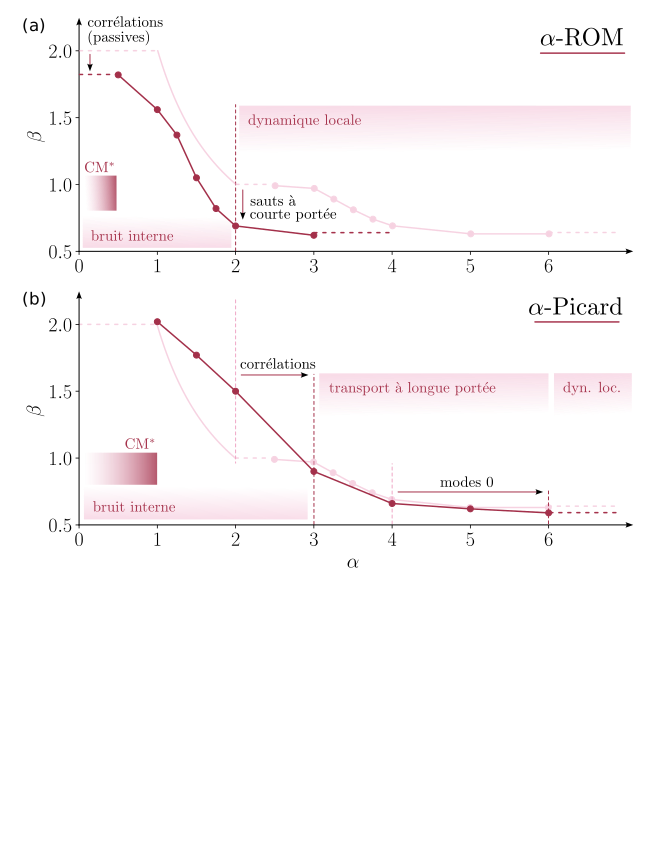
\includegraphics[width=0.9\textwidth]{Chapitre5/Figures/FigRecap.pdf}
	\caption{Figure récapitulative de l'étude comparée des transitions de réversibilité et d'écoulement, représentée via le prisme de l'évolution de l'exposant $\beta$ avec la portée $\alpha$ en 2D. (a) Cadres théoriques. Les points correspondent au mesures numériques sur le modèle LR-ROM (\autoref{chapter:TransportLP}). (b) Modèle $\alpha$-ROM (résultats du \autoref{chapter:Susp}). (c) Modèle $\alpha$-Picard (résultats du \autoref{chapter:yielding}).}
	\label{fig:Recap}
\end{figure}

\subsection{Conclusion de la section}

\subparagraph{}En conclusion, les transitions de réversibilité et d'écoulement étudiées à travers les modèles $\alpha$-Picard et $\alpha$-ROM présentent des similitudes frappantes. D'un point de vue constitutif, on y retrouve les mêmes ingrédients, similaires aux modèles de la classe CDP, et la présence d'interactions à longue portée ayant un effet spécifique. Celles-ci représentent un nouveau mécanisme de création de l'activité, associé à une diffusion vers un bord absorbant. D'un point de vue phénoménologique global, les deux transitions présentent les mêmes évolutions montrant un comportement critique atypique à très longue portée et un comportement similaire à l'universalité CDP à très courte portée. Nous remarquons par ailleurs dans ces deux modèles la présence d'un point singulier trivial mettant en lien le changement de convexité, l'inversement du comportement des fluctuations critiques et la perte de compacité spatiale des évènements dynamiques.


\subparagraph{}Toutefois, ces modèles présentent des points de divergence que l'on peut expliquer via deux cadres théoriques : le cadre LR-CDP qui rationalise l'influence du transport à longue portée et le cadre $\mu$-HL qui rationalise l'effet du bruit interne sur le comportement critique. De manière générale, nous pouvons mettre en avant deux différences fondamentales. La première est que le $\alpha$-ROM ne présente jamais de transport de la masse à longue portée alors que c'est le cas du modèle $\alpha$-Picard. La seconde est que les modèles d'écoulement font intervenir une forme très particulière du propagateur, induisant des fortes corrélations dans le système tandis que les modèles de particules présentent une dynamique simplifiée par le point de vue statistique.

\subparagraph{}Il pourrait nous être opposé que cette seconde différence vient d'un défaut de modélisation et qu'une approche plus réaliste des interactions hydrodynamiques dans le $\alpha$-ROM permettrait de l'effacer. Toutefois, toute l'importance de la forme du propagateur dans le cas du modèle $\alpha$-Picard réside dans le fait que tous les évènements plastiques sont alignés avec la direction de cisaillement principale (i.e. le propagateur de Eshelby a une direction unique). Dans le cas de la transition de réversibilité, il n'y a pas de fortes raisons de penser que cette orientation soit privilégiée, et que si chaque interaction est orientée aléatoirement les corrélation spatiales du propagateur ne sont pas importantes. Dans la \autoref{sec:ApproxScalaire}, nous présentons des résultats préliminaires qui confortent la faible importance de ces corrélations dans le cas du modèle de particules en proposant un traitement tensoriel des interactions dans celui-ci.

\subparagraph{}Finalement, l'étude comparée de ces deux transitions peut-être résumée par la \autoref{fig:Recap}.

\section{Équations de champ pour les transitions convexes}

\subsection{Motivations et difficultés}

\subparagraph{}Pour intégrer toute la complexité d'un phénomène critique dans une théorie simple, l'approche naturelle est celle des théories de champs. Via les méthodes du groupe de renormalisation, connaître la théorie de champ associée à un phénomène permet, en principe, d'en caractériser parfaitement la criticalité. Un exemple édifiant est celui de la transition de dépiégeage (et en définitive de la classe CDP) dont le traitement analytique a permis de nombreux progrès sur la compréhension du phénomène. Pour aller au-delà des descriptions champ moyen proposées par les modèles de type $\mu$-HL, il est donc naturel de vouloir déterminer une théorie de champ associée aux transitions convexes faisant intervenir une dynamique de bruit interne.

\subparagraph{}Cette motivation n'est en réalité pas nouvelle, autant du point de vue de la transition vers l'écoulement que du point de vue de la transition de réversibilité. En effet, du fait de sa proximité avec la transition de dépiégeage, certaines études ont cherché à établir une théorie continue homologue dans le cas de la transition vers l'écoulement \cite{tyukodi_depinning_2016, weiss_finite_2014}. Les équations proposées sont alors directement tirées des règles dynamiques des modèles élastoplastiques. Le problème est que celles-ci font intervenir la notion d'un seuil local, inadaptée à une approche macroscopique à grande échelle. Par ailleurs, l'introduction de l'interaction d'Eshelby dans une théorie continue sans seuil comme l'équation de quenched-Edward-Wilkinson pose problème, puisque la non-positivité du propagateur rend la procédure de renormalisation habituelle impossible \cite{wiese_blabla}. Une description continue adéquate manque donc toujours à la transition vers l'écoulement.

\subparagraph{}Du côté de la transition de réversibilité, l'étude menée par Mari et al. \cite{mari_absorbing_2022} avait mené à la suggestion d'une théorie de champ expliquant la convexité de la transition. Les auteurs ont proposé une traduction du mécanisme de diffusion vers l'activité comme une modification du terme non-linéaire en $\sim A^2$ dans l'équation CDP sur le champ d'activité en un terme en $\sim A^{3/2}$. Dans une approche champ moyen naïve, cela permet effectivement d'obtenir un exposant $\beta = 2$ et donc une transition convexe. Toutefois, si cette théorie était appuyée sur des arguments microscopiques, elle n'a jamais été testée afin de comprendre si cette convexité est effectivement retrouvée en dimension finie.

\subparagraph{}Il existe une tension entre cette recherche classique d'une théorie continue pour les transitions convexes et le cadre de champ moyen adapté que nous avons présenté précédemment avec les modèles de type Hébraud-Lequeux. En effet, il n'est pas évident de voir comment l'approche statistique sur la quantité conservée peut être traduite dans un langage de théorie de champ.

\subparagraph{}Dans cette section, nous présentons des résultats préliminaires obtenus sur cet axe de réflexion. Plus précisément nous essayons d'inférer des équations de champ adéquates pour reproduire la convexité de ces transitions, en se basant sur les théories de champ des classes CDP et LR-CDP. Pour tester ces équations, nous ne les étudions pas analytiquement mais plutôt numériquement en les intégrant directement. Ainsi, il est possible d'étudier les criticalités qu'elles décrivent de la même façon que les modèles microscopiques déjà considérés tout au long de cet ouvrage.

\subsection{Cadre de travail}

\subparagraph{}Établir une théorie de champ n'est de façon générale pas quelque chose d'évident, et encore moins lorsque l'on n'est pas spécialiste du domaine. Dans le cas des classes DP et CDP, les théories continues associées sont dérivées, plus ou moins directement, des processus de réaction-diffusion mentionnés dans le \autoref{chapter:introduction}. Dans notre cas, il est difficile d'imaginer un tel processus représentant l'effet du bruit interne sur la dynamique. Les systèmes que nous avons étudié ressemblant par de nombreux aspects aux modèles appartenant à la classe CDP, nous proposons de partir de la théorie continue la décrivant et d'en proposer des modifications. Pour rappel, celle-ci est représentée par les deux équations couplées suivantes :

\begin{equation}
\begin{aligned}
	&\partial_t A(\mathbf{r}, t) = (\omega\rho (\mathbf{r}, t) - r)A(\mathbf{r}, t) - uA^2(\mathbf{r}, t) + \kappa\Delta A (\mathbf{r}, t) + \sigma \sqrt{A(\mathbf{r}, t)} \eta(\mathbf{r}, t)\\
	&\partial_t \rho (\mathbf{r}, t) = \kappa\Delta A (\mathbf{r}, t)
\end{aligned}
\label{eq:CDP2}
\end{equation}

\noindent avec $A(\mathbf{r}, t)$ le champ d'activité et $\rho (\mathbf{r}, t)$ le champ conservé.

\subparagraph{}En principe, intégrer numériquement ces équations n'est pas chose simple, et ce pour une raison principale : dû à la présence du bruit dans l'équation sur l'activité, sans précaution particulière celle-ci peut devenir négative, ce qui est totalement proscrit. En théorie, les équations préservent la positivité de l'activité, mais en pratique, via un schéma d'intégration avec un pas de temps $\Delta t$ fini, celle-ci n'est pas assurée. Pour résoudre ce problème, nous utilisons un algorithme d'intégration proposé précédemment par Dornic et al. \cite{dornic_integration_2005}, permettant d'introduire le bruit multiplicatif tout en préservant la positivité de l'activité. Son principe et son implémentation sont détaillés à la \autoref{sec:Dornic}.

\subsection{Enjeux pratiques}

\subparagraph{}Dans cette sous-section, nous mettons en évidence les difficultés pratiques concernant l'établissement de telles théories de champ en prenant l'exemple représentatif de la transition vers l'écoulement.

\subparagraph{}Par équivalence avec la transition de dépiégeage, une théorie de champ intuitive pour la transition vers l'écoulement reviendrait à remplacer les termes en $\Delta A$ dans l'\autoref{eq:CDP2} par des convolutions avec le propagateur élastique de type Eshelby $\mathcal{G}\ast A$. Si cette formulation est en théorie valable pour l'équation sur la quantité conservée, elle pose un problème de principe dans le cas de l'équation sur l'activité. En effet, le propagateur associé présentant des parties négatives, cela signifie qu'une zone inactive caractérisée par $A = 0$ est susceptible de se voir attribuer une activité négative sous l'effet de cette interaction non-locale. Une solution intuitive à ce problème serait alors d'ajouter une partie locale à ce terme d'interaction afin qu'il prenne la forme $A\times \mathcal{G}\ast A$, assurant de ce fait que l'activité d'une zone inactive ne puisse pas être diminuée. Toutefois cela pose un second problème : dans ce cadre, une zone inactive ne peut pas être activée à distance (puisque le terme d'interaction à longue portée associé est nul), ce qui constitue un aspect essentiel du mécanisme que l'on cherche à modéliser.

\subparagraph{}La dynamique de bruit interne semblant devoir faire intervenir des interactions à longue portée de signes alternés (i.e. capables de favoriser comme de défavoriser la création d'activité), cette difficulté se retrouve dans toutes les théories intuitives que l'on peut proposer pour les différentes transitions. Les équations de champ que nous avons envisagées permettent donc toutes de répondre à ces deux critères :

\begin{itemize}
	\item faire intervenir des interactions capables de créer de l'activité dans des zones inactives à longue portée
	\item faire intervenir des interactions inhibitrices de l'activité à longue portée préservant la positivité de l'activité en tout point.
\end{itemize}

\subsection{Résultats préliminaires}

\subparagraph{}Dans cette section, nous présentons des théories que nous avons envisagé dans le cadre de la modélisation des transitions de réversibilité et d'écoulement. Les résultats préliminaires que nous avons obtenus montrent que les formulations intuitives des équations de champ pour modéliser les transitions convexes sont inadéquates. Plus particulièrement, nous montrons qu'avec des interactions associées à longue portée, celles-ci ne permettent pas de dépasser le paradigme $\beta \approx 1$. Afin de ne pas tomber dans l'écueil de présenter exhaustivement toutes nos tentatives non fructueuses, nous proposons dans cette sous-section de présenter simplement trois théories motivées par les modèles microscopiques que nous avons étudié dans cet ouvrage.

\subsubsection{Exemple de théorie motivée par le modèle de Picard}

\subparagraph{}Dans le cadre de la modélisation continue du modèle de Picard, une théorie envisageable est celle représentée par les équations suivantes :

\begin{equation}
    \begin{aligned}
        \partial_t A (\mathbf{r}, t) &= \left(\omega \rho (\mathbf{r}, t)-r\right) A (\mathbf{r}, t) - uA^2 (\mathbf{r}, t) + \kappa \left(\mathcal{G}^+\ast A \right)(\mathbf{r}, t) + \kappa\left(\mathcal{G}\ast A \right)(\mathbf{r}, t)A (\mathbf{r}, t) \\
        &+\sigma \sqrt{A (\mathbf{r}, t)}\eta(\mathbf{r}, t)\\
        \partial_t \rho (\mathbf{r}, t) &= \kappa_\sigma \left(\mathcal{G}\ast A \right)(\mathbf{r}, t)
    \end{aligned}
\label{eq:YieldingD}
\end{equation}

\noindent avec $\mathcal{G}$ le porpagateur d'Eshelby et $\mathcal{G}^+$ sa partie positive définie selon :

\begin{equation}
	\mathcal{G}^+(\mathbf{r}) = \mathcal{G}(\mathbf{r})\Theta\left(\mathcal{G}(\mathbf{r})\right)
\end{equation}

\noindent avec $\Theta$ la fonction de Heaviside. Sous cette formulation, les deux critères énoncés précédemment sont respectés : le terme en $\sim \mathcal{G}^+\ast A$ permet une création à distance d'activité dans les zones inactives et le terme en $A\times \mathcal{G}\ast A$ permet une inhibition de l'activité à distance tout en préservant sa positivité.

\subparagraph{}En variant la valeur du paramètre $r$, l'intégration numérique de ces équations révèle bien la présence d'une transition de phase absorbante. Pour $r>r_c$, le système se stabilise à temps long dans un état stationnaire caractérisé par $\langle A \rangle > 0$ alors que pour $r<r_c$ il finit par tomber dans un état absorbant caractérisé par $A = 0$. Toutefois, en analysant l'évolution de l'activité en fonction de la distance au point critique $\delta r$, nous remarquons que cette transition semble caractérisée trivialement par $\beta \approx 1$, comme cela est illustré à la \autoref{fig:YieldingD}. D'après ces résultats préliminaires, cette formulation ne semble donc pas permettre de retranscrire la convexité de la transition et donc le processus de bruit interne inhérent à la dynamique modélisée.

\begin{figure}[h]
	\centering
	\includegraphics[width=\textwidth]{Chapitre5/Figures/YieldingD.pdf}
	\caption{Intégration numérique de l'\autoref{eq:YieldingD} dans un système 2D de taille $L=512$ avec comme valeur des paramètres : $\omega = 1$, $u = 1$, $\kappa = 0.25$, $\kappa_\sigma = 0.25$, $\sigma = 1$ et une valeur moyenne du champ conservé $\bar{\rho} = 1$. Le paramètre $r$ est varié dans l'ensemble $\{ 0.5214,  0.6153, 0.6726, 0.7076, 0.7290, 0.7420, 0.7500, 0.7549\}$. (a) Evolution de la valeur moyenne du champ d'activité en fonction du temps pour des différentes valeurs du paramètre $r$. (b) Evolution de la valeur moyenne de l'activité dans l'état stationnaire en fonction de la distance au point critique $\delta r$. Nous estimons ici $r_c \approx 0.7625$.}
	\label{fig:YieldingD}
\end{figure}

\subsubsection{Exemple de théorie motivée par le modèle $\alpha$-ROM}

\subparagraph{}Dans l'étude menée par Mari et al. \cite{mari_absorbing_2022} sur le $0$-ROM, les auteurs ont proposé une théorie continue dérivée de celle de CDP en y introduisant un terme de création d'activité dû à la diffusion des particules passives. Dans le cadre d'interactions spatialisées comme nous avons considéré dans le cas du $\alpha$-ROM, cette théorie continue peut se généraliser simplement par la forme suivante (voir \autoref{sec:EqChampROM}) :

\begin{equation}
    \begin{aligned}
        \partial_t A (\mathbf{r}, t) &= \left(\omega \rho (\mathbf{r}, t)-r\right) A (\mathbf{r}, t) - uA^2 (\mathbf{r}, t) +\kappa \Delta A (\mathbf{r}, t)\\
        &+ \kappa \left(G\ast A \right)(\mathbf{r}, t)\left(1-\gamma \sqrt{ \left(G\ast A \right)(\mathbf{r}, t)}\right)\rho (\mathbf{r}, t)+ \sigma \sqrt{A (\mathbf{r}, t)}\eta (\mathbf{r}, t)\\
        \partial_t \rho (\mathbf{r}, t) &= \kappa_\sigma \Delta A (\mathbf{r}, t)
    \end{aligned}
\label{eq:SuspensionsB}
\end{equation}

\noindent avec $G(\mathbf{r})$ un propagateur positif décroissant comme $\sim 1/r^{2\alpha}$ à grande distance. En pratique, nous considérons le même propagateur que dans les modèles $\alpha$-ROM et conservons son implémentation décrite au \autoref{chapter:Susp}.

\subparagraph{}Afin de voir si cette formulation permet de reproduire la convexité de la transition, nous intégrons ces équations stochastiques pour différentes valeurs de $r$. Nous retrouvons alors une transition de phase absorbante dont la caractérisation préliminaire est présentée sur la \autoref{fig:SuspensionsB}. Via une analyse similaire au cas précédent, nous déterminons $\beta \approx 1.09$ pour $\alpha = 0.5$, la valeur $\beta = 1$ étant comprise dans les incertitudes de détermination. \`A cette valeur de la portée, nous sommes dans la limite de portée infinie du $\alpha$-ROM caractérisée précédemment par $\beta \approx 1.85$. Ce résultat $\beta \approx 1$ suggère donc que cette théorie continue ne permet pas non plus d'expliquer la convexité de la transition dans le modèle de particules.

\begin{figure}[h]
	\centering
	\includegraphics[width=\textwidth]{Chapitre5/Figures/SuspensionsB.pdf}
	\caption{Intégration numérique de l'\autoref{eq:SuspensionsB} dans un système 2D de taille $L=1024$ avec comme valeur des paramètres : $\omega = 0.04$, $u = 1$, $\kappa = 0.25$, $\kappa_\sigma = 0.01$, $\sigma = 1$, $\gamma = 0.1$ et une valeur moyenne du champ conservé $\bar{\rho} = 25$. Le paramètre $r$ est varié dans l'ensemble $\{ 0.602, 0.711, 0.777, 0.816, 0.842, 0.857, 0.867, 0.872\}$. (a) Evolution de la valeur moyenne du champ d'activité en fonction du temps pour des différentes valeurs du paramètre $r$. (b) Evolution de la valeur moyenne de l'activité dans l'état stationnaire en fonction de la distance au point critique $\delta r$. Nous estimons ici $r_c \approx 0.8813$.}
	\label{fig:SuspensionsB}
\end{figure}

\subsubsection{Approche naïve via l'attendu champ moyen}

\subparagraph{}Face aux difficultés posées par la prise en compte d'interactions à longue portée non-monotones, nous pouvons imaginer une autre voie vers la convexité via la modification des termes locaux de la théorie de champ CDP. C'est notamment l'idée déjà proposée par Mari et al. \cite{mari_absorbing_2022} qui considère les équations de champ suivantes dans le cas d'une portée d'interaction infinie :

\begin{equation}
\begin{aligned}
	&\partial_t A(\mathbf{r}, t) = (\omega\rho (\mathbf{r}, t) - r)A(\mathbf{r}, t) - uA^{3/2}(\mathbf{r}, t) + \kappa\Delta A (\mathbf{r}, t) + \sigma \sqrt{A(\mathbf{r}, t)} \eta(\mathbf{r}, t)\\
	&\partial_t \rho (\mathbf{r}, t) = \kappa\Delta A (\mathbf{r}, t)
\end{aligned}
\label{eq:CDP32}
\end{equation}

\noindent Dans une approche habituelle de la théorie de champ moyen qui équivaut à négliger les termes de bruit et d'interaction, cette théorie amène en effet à un exposant $\beta^\text{MF} = 2$.

\subparagraph{}Pour comprendre si cette formulation permet effectivement de retrouver une transition convexe caractérisée par $\beta > 1$, nous intégrons l'\autoref{eq:CDP32} dans sa forme champ moyen. Pour ce faire, le terme d'interaction local $\Delta A$ est remplacé par $\bar{A}-A$ avec $\bar{A}$ la valeur moyenne instantanée du champ d'activation. Toujours en faisant varier le paramètre $r$, nous observons une transition de phase absorbante mais dont la criticalité semble être encore caractérisée par $\beta \approx 1$, comme nous le représentons à la \autoref{fig:MFCDP32}. Bien que ces résultats restent préliminaires, cette étude présente une approche du point critique raisonnable qui suggère que la transition n'est effectivement pas convexe dans la limite de très longue portée.

\subparagraph{}Même si cela peut apparaître surprenant, dans la \autoref{sec:Munoz}, nous montrons que ce résultat est en fait prévisible d'un point de vue analytique. Comme des études précédentes l'ont montré, les théories de champ faisant intervenir des bruits multiplicatifs ne possèdent pas des propriétés champ moyen dérivables trivialement \cite{munoz_mean_field_2005, munoz_multiplicative_2003}. \`A la place, un autre traitement du champ moyen doit être opéré. Celui-ci mène alors à un exposant $\beta^\text{MF} = 1$ quel que soit le degré de non-linéarité choisi dans une théorie présentant un terme de bruit multiplicatif en $\sim \sqrt{A(\mathbf{r}, t)}$.

\begin{figure}[h]
	\centering
	\includegraphics[width=\textwidth]{Chapitre5/Figures/MFCDP32.pdf}
	\caption{Intégration numérique de l'\autoref{eq:CDP32} dans un système 2D de taille $L=1024$ avec comme valeur des paramètres : $\omega = 1$, $u = 0.5$, $\kappa = 0.25$, $\kappa_\sigma = 0.01$, $\sigma = 1$, $\gamma = 0.1$ et une valeur moyenne du champ conservé $\bar{\rho} = 1$. Le paramètre $r$ est varié dans l'ensemble $\{ 0.2462, 0.3010, 0.3295, 0.3442, 0.3518, 0.3558, 0.3578, 0.3589\}$. (a) Evolution de la valeur moyenne du champ d'activité en fonction du temps pour des différentes valeurs du paramètre $r$. (b) Evolution de la valeur moyenne de l'activité dans l'état stationnaire en fonction de la distance au point critique $\delta r$. Nous estimons ici $r_c \approx 0.36083$.}
	\label{fig:MFCDP32}
\end{figure}

\subsection{Conclusion de la section}

\subparagraph{}En conclusion, il ne semble pas aisé de mettre en évidence des équations de champ permettant de produire une transition de phase absorbante convexe. Que ce soit via l'introduction d'interactions à longue portée de signe alterné, l'introduction d'une non-analyticité dans le terme non-local ou la modification du degré de non-linéarité du terme non-linéaire local, le comportement critique dans la limite de longue portée semble être toujours limité à $\beta = 1$. Les tests d'intégration que nous avons présenté ici sont les représentants de nombreux autres essais pointant vers le même résultat. 

\subparagraph{}Ces difficultés suggèrent que le cadre représenté par les équations de type CDP/LR-CDP n'est pas le bon point de départ. Pour poursuivre dans cette direction, il faudrait donc considérer des modifications plus profondes de ces théories afin d'appréhender plus justement le mécanisme de diffusion vers un bord absorbant, qui est l'élément central de ces transitions. Nous pourrions imaginer que cette modélisation passe par la considération d'une nouvelle forme de bruit non-locale, celle d'une dynamique d'un champ complémentaire représentant la distance au bord absorbant ou encore celle d'une complexification de l'équation sur la dynamique du champ conservé. Notons par ailleurs que la modification de la forme du bruit dans l'équation sur l'activité ou l'ajout d'un bruit dans la dynamique du champ conservé ne sont pas des éléments directs à implémenter et nécessitent la modification de tout notre schéma numérique. Une telle investigation gagnerait donc à être sérieusement motivée par des arguments émergents des dynamiques microscopiques.

\subparagraph{}La différence de formulation entre ces théories de champs et les modèle à la Hébraud-Lequeux pourrait être un indice de ces potentielles profondes modifications. Une autre piste d'ouverture pourrait donc être d'essayer de réaliser une équivalence entre ces modèles et une équation de champ triviale dans la limite de champ moyen. \`A ce stade de notre recherche, nous n'avons toutefois pas encore pu explorer cette pistes de manière pertinente.

%\section{Notes random}
%
%Je prends des notes ici sur les trucs qui me viennent pendant que je rédige les autres chapitres :
%
%\begin{itemize}
%	\item Peut-on toujours dire que les champs conservés sont non-diffusifs ? On sait qu'au niveau théorie de champ ça change bcp de choses que le champ soit diffusif ou non, même si niveau champ moyen ça change rien.. Peut-être que ça vaut le coup d'au moins le mentionner.
%	\item Une différence entre le yielding et les suspensions est que pour les suspensions on démarre l'influence du bruit à partir de de la courte portée. Dans le cas du yielding, le bruit commence à avoir une influence (théorie type LHL) à partir du champ moyen type depinning. C'est notamment surement pour ça qu'on n'a pas les mêmes évolutions de l'HU.
%	\item Comparer yielding et depinning pour $\beta <1$ serait intéressant, en plus d'être numériquement pas si exigeant.
%	\item si on a bien un scénario du type LR-CDP puis LHL pour le yielding, c'est assez fou que l'évolution soit aussi continue... (après peut-on vraiment voir deux régimes avec si peu de points)
%	\item Même si numériquement ça fonctionne pas du tout, la coincidence entre $d =d_f$ et $\beta$ qui devient plus grand que 1 ou gamma prime plus petit que 0 peut se voir en utilisant le scaling de Lin et Wyart.
%	\item Vu qu'on a attribué la dépendance en protocole au P(x) selon Jagla, est-ce qu'elle disparait à courte portée ? Oui.
%	\item A priori si la relation $d_f = D + \eta$ est valable pour l'AQS on aura aussi un changement de $d_f$ avec des avalanches type AQS.
%	\item Yielding et suspensions sont différents par le fait que le yielding fait aussi de la redistribution de masse à LP.
%	\item Dans la littérature on dit que pour Manna les avalanches c'est pareil à densité imposée qu'en SOC. Est-ce que c'est vrai aussi en LP canonique ? Probablement vérifiable. Probablement pas vrai en LP médiée ! Dans ce cas là, notre résultats sur les avalanches EPM peut avoir un impact plus grand que celui escompté au départ.
%\end{itemize}
%
%\section{Points de discussion (mais pas à mettre dans la discussion)}
%
%\begin{itemize}
%	\item Janseen et al. disent que $\sigma_c$ est en fait légèrement différent de $2$ dans DP, pourquoi ça ne pourrait pas être le cas dans CDP ? Il y a une justification du côté du depinning ? Oui d'après Kay mais j'ai pas compris ce qu'il a dit.
%\end{itemize}
%
%\subsection{De nouvelles interrogations}
%
%Question un peu ouvertes, juste des connexions que j'aimerais mentionner pour pas les oublier
%
%\begin{itemize}
%	\item suggérer que avalanches après chargement et avalanches à densité fixée c'est pas évident que ça sera pareil dans les suspensions.
%	\item Remarques sur $\beta = 1$ qui correspond à $d_f = D$ et autre.
%\end{itemize}
